\section{Trigonometric Substitutions}{}{}\label{sec:Trig Sub}
So far we have seen that it sometimes helps to replace a subexpression
of a function by a single variable. Occasionally it can help to
replace the original variable by something more complicated. This
seems like a ``reverse'' substitution, but it is really no different
in principle than ordinary substitution.

\begin{example}{Sine Subsitution}{Sine Subsitution}
Evaluate $\ds\int \sqrt{1-x^2}\,dx$. 
\end{example}

\begin{solution}
Let $x=\sin u$ so 
$dx=\cos u\,du$. Then
$$
  \int \sqrt{1-x^2}\,dx=\int\sqrt{1-\sin^2 u}\cos u\,du=
  \int\sqrt{\cos^2 u}\cos u\,du.
$$
We would like to replace $\ds \sqrt{\cos^2 u}$ by $\cos u$, but this is
valid only if $\cos u $ is positive, since $\ds \sqrt{\cos^2 u}$ is
positive. Consider again the substitution $x=\sin u$. We could just as
well think of this as $u=\arcsin x$. If we do, then by the definition
of the arcsine, $-\pi/2\le u\le\pi/2$, so $\cos u\ge0$. Then we
continue:
\begin{eqnarray*}
  \int\sqrt{\cos^2 u}\cos u\,du&=&\int\cos^2u\,du\\
	&=&\int {1+\cos 2u\over2}\,du = {u\over 2}+{\sin 2u\over4}+C\cr
  &=&{\arcsin x\over2}+{\sin(2\arcsin x)\over4}+C.
\end{eqnarray*}
This is a perfectly good answer, though the term
$\sin(2\arcsin x)$ is a bit unpleasant. It is possible to simplify
this. Using the identity $\sin 2x=2\sin x\cos x$, we can write
$\ds \sin 2u=2\sin u\cos u=2\sin(\arcsin x)\sqrt{1-\sin^2 u}=
2x\sqrt{1-\sin^2(\arcsin x)}=2x\sqrt{1-x^2}.$ Then the full
antiderivative is 
$$
  {\arcsin x\over2}+{2x\sqrt{1-x^2}\over4}=
  {\arcsin x\over2}+{x\sqrt{1-x^2}\over2}+C.
$$
\end{solution}

This type of substitution is usually indicated when the function you
wish to integrate contains a polynomial expression that might allow
you to use the fundamental identity $\ds \sin^2x+\cos^2x=1$ in
one of three forms:
$$
  \cos^2 x=1-\sin^2x
  \qquad
  \sec^2x=1+\tan^2x
  \qquad
  \tan^2x=\sec^2x-1.
$$
If your function contains $\ds 1-x^2$, as in the example above, try
$x=\sin u$; if it contains $\ds 1+x^2$ try $x=\tan u$; and if it contains
$\ds x^2-1$, try $x=\sec u$. Sometimes you will need to try something a
bit different to handle constants other than one which we will describe below.
First we discuss inverse substitutions.

In a {\bf traditional} substitution we let $u=u(x)$, i.e., our new variable is defined in terms of $x$.  
In an {\bf inverse} substitution we let $x=g(u)$, i.e., we assume $x$ can be written in terms of $u$.  
We cannot do this arbitrarily since we do \thmfont{NOT} get to ``choose'' $x$.
For example, an inverse substitution of $x=1$ will give an obviously wrong answer.  
However, when $x=g(u)$ is an invertible function, then we are really doing a $u$-substitution with $u=g^{-1}(x)$.  
Now the substitution rule applies.

Sometimes with inverse substitutions involving trig functions we use $\theta$ instead of $u$. 
Thus, we would take $x=\sin\theta$ instead of $x=\sin u$. 
However, as we discussed above, we would like our inverse substitution $x=g(u)$ to be a one-to-one function, and $x=\sin u$ is not one-to-one.
We can overcome this issue by using the restricted trigonometric functions.
The three common trigonometric substitutions are the restricted sine, restricted tangent and restricted secant.
Thus, for sine we use the domain $[-\pi/2,~\pi/2]$ and for tangent we use $(-\pi/2,~\pi/2)$.
Depending on the convention chosen, the restricted secant function is usually defined in one of two ways.
$$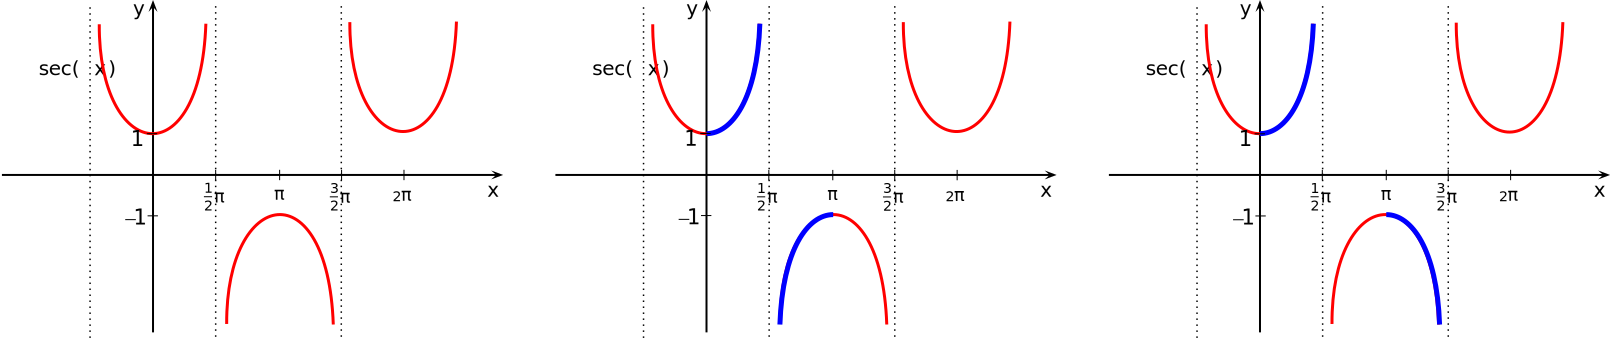
\includegraphics[width=6in]{images2/inv-trig-sec}$$
One convention is to restrict secant to the region $[0,~\pi/2)\cup(\pi/2,\pi]$ as shown in the middle graph.
The other convention is to use $[0,~\pi/2)\cup[\pi,~3\pi/2)$ as shown in the right graph.
Both choices give a one-to-one restricted secant function and no universal convention has been adopted.
To make the analysis in this section less cumbersome, we will use the domain $[0,~\pi/2)\cup[\pi,~3\pi/2)$ for the restricted secant function.
Then $\sec^{-1}x$ is defined to be the inverse of this restricted secant function.

Typically trigonometric substitions are used for problems that involve radical expressions.
The table below outlines when each substitution is typically used along with their intervals of validity.


%$$\begin{array}{|c|c|c|}
%\hline
%\mbox{\thmfont{Expression}} & \mbox{\exfont{Substitution}} & \mbox{\deffont{Validity}}\\
%\hline ~ & ~ & ~ \\
%\sqrt{a^2-x^2} & x=a\sin\theta & \theta\in[-\pi/2,~\pi/2]\\
%~ & ~ & ~ \\\hline~ & ~ & ~ \\
%\sqrt{a^2+x^2}~~\mbox{or}~~a^2+x^2 & x=a\tan\theta & \theta\in(-\pi/2,~\pi/2)\\
%~ & ~ & ~ \\\hline~ & ~ & ~ \\
%\sqrt{x^2-a^2} & x=a\sec\theta & \theta\in[0,~\pi/2)\cup[\pi,~3\pi/2)\\
%~ & ~ & ~ \\\hline
%\end{array}$$

\begin{formulabox}[Trigonometric Substitution]
\begin{enumerate}
	\item[(a)] \noindent%
		\begin{minipage}[t]{.6\linewidth}%
		For integrands containing $\sqrt{a^2-x^2}$:\index{integration!trig. subst.}\\[5pt]
		Let $x=a\sin\theta$, \qquad $dx = a\cos\theta\ d\theta$\\[5pt]	
	Thus $\theta = \sin^{-1}(x/a)$, for $-\pi/2\leq \theta\leq \pi/2$. \\[5pt]	
	On this interval, $\cos\theta\geq 0$, so\\[5pt]	
	$\sqrt{a^2-x^2} = a\cos\theta$
		\end{minipage}\qquad
	\begin{minipage}[t]{.4\linewidth}\vskip 0pt
		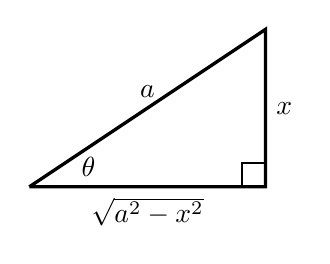
\begin{tikzpicture}
				\draw [very thick] (0,0) -- node[below,pos=.5] { $\sqrt{a^2-x^2}$} (3,0) -- node [right,pos=.5] { $x$} (3,2) -- node [pos=.5,above] { $a$} (0,0);
				\draw [thick] (2.7,0) -- (2.7,.3) -- (3,.3);
				\draw (.75,.25) node {$\theta$};		
		\end{tikzpicture}
		\end{minipage}
		
	\item[(b)] \noindent
	\begin{minipage}[t]{.6\linewidth}
		For integrands containing $\sqrt{x^2+a^2}$:\\[5pt]
		Let $x=a\tan\theta$, \qquad $dx = a\sec^2\theta\ d\theta$\\[5pt]	
	Thus $\theta = \tan^{-1}(x/a)$, for $-\pi/2 < \theta < \pi/2$. \\[5pt]	
	On this interval, $\sec\theta> 0$, so\\[5pt]	
	$\sqrt{x^2+a^2} = a\sec\theta$
		\end{minipage}\qquad
	\begin{minipage}[t]{.4\linewidth}\vskip 0pt
	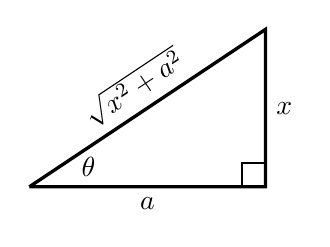
\begin{tikzpicture}
			\draw [very thick] (0,0) -- node[below,pos=.5] { $a$} (3,0) -- node [right,pos=.5] { $x$} (3,2) -- node [pos=.5,above,sloped] { $\sqrt{x^2+a^2}$} (0,0);
			\draw [thick] (2.7,0) -- (2.7,.3) -- (3,.3);
			\draw (.75,.25) node {$\theta$};	
	\end{tikzpicture}
		\end{minipage}
		
	\item[(c)] \noindent
	\begin{minipage}[t]{.6\linewidth}
		For integrands containing $\sqrt{x^2-a^2}$:\\[5pt]
		Let $x=a\sec\theta$, \qquad $dx = a\sec\theta\tan\theta\ d\theta$\\[5pt]	
	Thus $\theta = \sec^{-1}(x/a)$. If $x/a\geq 1$, then $0\leq\theta<\pi/2$; if $x/a \leq -1$, then $\pi\le\theta< 3\pi/2$.\\[5pt]	
	We restrict our work to where $x\geq a$, so $x/a\geq 1$, and $0\leq\theta<\pi/2$.
	On this interval, $\tan\theta\geq 0$, so\\[5pt]	
	$\sqrt{x^2-a^2} = a\tan\theta$
		\end{minipage}\qquad
	\begin{minipage}[t]{.4\linewidth}\vskip 0pt
		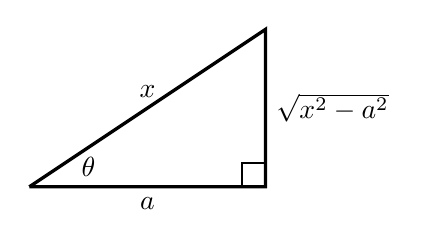
\begin{tikzpicture}
				\draw [very thick] (0,0) -- node[below,pos=.5] { $a$} (3,0) -- node [right,pos=.5] { $\sqrt{x^2-a^2}$} (3,2) -- node [pos=.5,above] { $x$} (0,0);
				\draw [thick] (2.7,0) -- (2.7,.3) -- (3,.3);
				\draw (.75,.25) node {$\theta$};			
		\end{tikzpicture}
		\end{minipage}	
\end{enumerate}

\end{formulabox}

All three substitutions are one-to-one on the listed intervals.
When dealing with radicals we often end up with absolute values since
$$\sqrt{z^2}=|z|.$$
For each of the three trigonometric substitions above we will verify that we can ignore the absolute value in each case when encountering a radical.

For $x=a\sin\theta$, the expression $\sqrt{a^2-x^2}$ becomes
$$\sqrt{a^2-x^2}
= \sqrt{a^2-a^2\sin^2\theta}
= \sqrt{a^2(1-\sin^2\theta)}
= a\sqrt{\cos^2\theta}
= a|\cos\theta|
= a\cos\theta$$ 
This is because $\cos\theta\geq 0$ when $\theta\in[-\pi/2,~\pi/2]$. 
For $x=a\tan\theta$, the expression $\sqrt{a^2+x^2}$ becomes
$$\sqrt{a^2+x^2}
= \sqrt{a^2+a^2\tan^2\theta}
= \sqrt{a^2(1+\tan^2\theta)}
= a\sqrt{\sec^2\theta}
= a|\sec\theta|
= a\sec\theta$$ 
This is because $\sec\theta>0$ when $\theta\in(-\pi/2,~\pi/2)$. 

Finally, for $x=a\sec\theta$, the expression $\sqrt{x^2-a^2}$ becomes
$$\sqrt{x^2-a^2}
= \sqrt{a^2\sec^2\theta-a^2}
= \sqrt{a^2(\sec^2\theta-1)}
= a\sqrt{\tan^2\theta}
= a|\tan\theta|
= a\tan\theta$$
This is because $\tan\theta\geq 0$ when $\theta\in[0,~\pi/2)\cup[\pi,~3\pi/2)$. 

Thus, when using an appropriate trigonometric substitution we can usually ignore the absolute value. 
After integrating, we typically get an answer in terms of $\theta$ (or $u$) and need to convert back to $x$'s.
To do so, we use the two guidelines below:
\begin{itemize}
	\item For trig functions containing $\theta$, use a triangle to convert to $x$'s.
	\item For $\theta$ by itself, use the inverse trig function.
\end{itemize}

All pieces needed for such a trigonometric substitution can be summarized as follows:
\[\begin{array}{|c|c|c|c|c|}\hline	%5 columns
		&	&	&	&	\text{\textbf{Inverse of}}	\\
\text{\textbf{Expression}}	&	\text{\textbf{Substitution}}	&	\text{\textbf{Differential}}	&	\text{\textbf{Identity}}	&	\text{\textbf{Substitution}}	\\	\hline
~	&	~	&	~	&	~	&	~	\\
\sqrt{a^2-x^2}	&	x=a\sin\theta	&	dx=a\cos\theta d\theta	&	\sqrt{a^2-x^2}=a\cos\theta	&	\theta=\sin^{-1}\left(\frac{x}{a}\right)	\\
~	&	~	&	~	&	~	&	~	\\	\hline
~	&	~	&	~	&	~	&	~	\\
\sqrt{a^2+x^2}	&	&	&	&	\\
 \text{or} 	&	x=a\tan\theta	&	dx=a\sec^2\theta d\theta	&	\sqrt{a^2+x^2}=a\sec\theta	&	\theta=\tan^{-1}\left(\frac{x}{a}\right)	\\
a^2+x^2 	&	&	&	&	\\
~	&	~	&	~	&	~	&	~	\\	\hline
~	&	~	&	~	&	~	&	~	\\
\sqrt{x^2-a^2}	&	x=a\sec\theta	&	dx=a\sec\theta\tan\theta d\theta	&	\sqrt{x^2-a^2}=a\tan\theta	&	\theta=\sec^{-1}\left(\frac{x}{a}\right)	\\
~	&	~	&	~	&	~	&	~	\\	\hline
\end{array}\]

To emphasize the technique, we redo the computation for $\ds\int \sqrt{1-x^2}\,dx$.

\begin{example}{Sine Subsitution}{Sine Subsitution}
Evaluate $\ds\int \sqrt{1-x^2}\,dx$. 
\end{example}

\begin{solution}
Since $\sqrt{1-x^2}$ appears in the integrand we try the trigonometric substitution $x=\sin\theta$.
(Here we are using the restricted sine function with $\theta\in[-\pi/2,~\pi/2]$ but typically omit this detail when writing out the solution.)
Then $\fbox{$dx$}=\fbox{$\cos \theta\,d\theta$}$.  
$$\begin{array}{>{\displaystyle}r>{\displaystyle}c>{\displaystyle}l>{\displaystyle}l}
	\int \sqrt{1-x^2}\,\fbox{$dx$} & = & \int\sqrt{1-\sin^2\theta}\,\fbox{$\cos \theta\,d\theta$} &\mbox{Using our (inverse) substitution}\\  
	& = & \int \sqrt{\cos^2\theta}\cos \theta\,d\theta &\mbox{Since $\sin^2\theta+\cos^2\theta=1$}\\  
	& = & \int |\cos\theta|\cdot\cos\theta\,d\theta & \mbox{Since $\sqrt{\cos^2\theta}=|\cos\theta|$}\\  
	& = & \int \cos^2\theta\,d\theta & \mbox{Since for $\theta\in[-\frac{\pi}{2},\frac{\pi}{2}]$ we have $\cos\theta\geq0$.}\\  
\end{array}$$
Often we omit the step containing the absolute value by our discussion above.
Now, to integrate a power of cosine we use the guidelines for products of sine and cosine and make use of the identity 
 $$\cos^2\theta=\frac{1}{2}(1+\cos(2\theta)).$$
Our integral then becomes
$$\int \sqrt{1-x^2}\,dx=\frac{1}{2}\int (1+\cos(2\theta))\,d\theta=\frac{\theta}{2}+\frac{\sin(2\theta)}{4}+C$$
To write the answer back in terms of $x$ we first use the identity $ \sin(2\theta) = 2\sin\theta \cos\theta $. So
$$\int \sqrt{1-x^2}\,dx= \frac{\theta}{2}+\frac{\sin(\theta)\cos(\theta)}{2}+C$$

%$$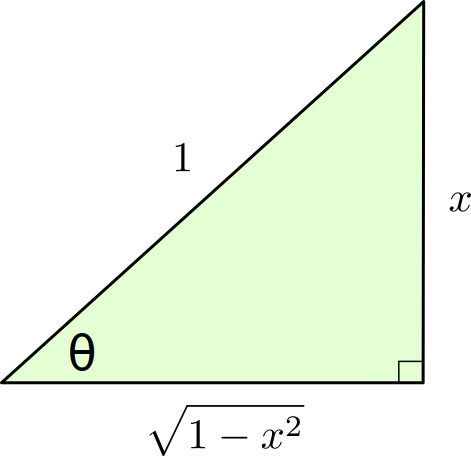
\includegraphics[width=1.65in]{images2/inv-trig-triangle-1}$$ 
\begin{minipage}{.7\textwidth}
Since	 $x=\sin\theta$, we can build the corresponding triangle and use SOH CAH TOA  we get $ \cos\theta = \frac{\sqrt{1-x^2}}{1} = \sqrt{1-x^2}.$
	This gives
	$$\int \sqrt{1-x^2}\,dx =\frac{\sin^{-1}x}{2}+\frac{x\sqrt{1-x^2}}{2}+C$$
\end{minipage}
\begin{minipage}{.3\textwidth}
	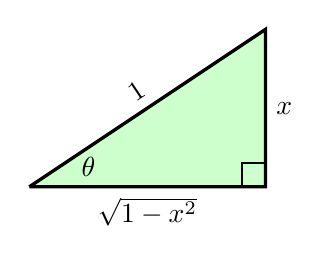
\begin{tikzpicture}
	\draw [very thick, fill=green!20] (0,0) -- node[below,pos=.5] { $\sqrt{1-x^2}$} (3,0) -- node [right,pos=.5] { $x$} (3,2) -- node [pos=.5,above,sloped] { $ 1 $} (0,0);
	\draw [thick] (2.7,0) -- (2.7,.3) -- (3,.3);
	\draw (.75,.25) node {$\theta$};	
	\end{tikzpicture}
\end{minipage}

\end{solution}

\begin{example}{Secant Subsitution}{Secant Subsitution} 
Evaluate $\ds\int\frac{\sqrt{25x^2-4}}{x}\,dx$.
\end{example}

\begin{solution}
We do not have $\sqrt{x^2-a^2}$ because of the $25$, but if we factor $25$ out we get: 
$$\ds\int\frac{\sqrt{25(x^2-(4/25))}}{x}\,dx=\ds\int5\frac{\sqrt{x^2-(4/25)}}{x}\,dx.$$
Now, $a=2/5$, so let $x=\frac{2}{5}\sec\theta$. 
Alternatively, we can think of the integral as being:
$$\ds\int\frac{\sqrt{(5x)^2-4}}{x}\,dx$$ 
Then we could let $u=5x$ followed by $u=2\sec\theta$, etc. 
Or equivalently, we can avoid a $u$-substitution by letting $5x=2\sec\theta$. 
In either case we are using the trigonometric substitution $x=\frac{2}{5}\sec\theta$, but do use the method that makes the most sense to you!
As $x=\frac{2}{5}\sec\theta$ we have $\fbox{$dx$}=\fbox{$\frac{2}{5}\sec\theta\tan\theta\,d\theta$}$.  
$$\begin{array}{>{\displaystyle}r>{\displaystyle}c>{\displaystyle}l>{\displaystyle}l}
	\int\frac{\sqrt{25x^2-4}}{x}\,\fbox{$dx$} & = & \int \frac{\sqrt{25\frac{4\sec^2\theta}{25}-4}}{\frac{2}{5}\sec\theta}\,\fbox{$\frac{2}{5}\sec\theta\tan\theta\,d\theta$} &\mbox{Using the substitution}\\  
	& = & \int\sqrt{4(\sec^2\theta-1)}\cdot \tan\theta\,d\theta & \mbox{Cancelling}\\ 
	& = & 2\int\sqrt{\tan^2\theta}\cdot \tan\theta\,d\theta & \mbox{Using $\tan^2\theta+1=\sec^2\theta$}\\ 
	%& = & 2\int\tan\theta\cdot \tan\theta\,d\theta & \mbox{Since $\sqrt{\tan^2\theta}=|\tan\theta|=\tan\theta$}\\ 
	& = & 2\int\tan^2\theta\,d\theta & \mbox{Simplifying}\\ 
	& = & 2\int(\sec^2\theta-1)\,d\theta & \mbox{Using $\tan^2\theta+1=\sec^2\theta$}\\ 
	& = & 2(\tan\theta-\theta)+C & \mbox{Since $\ds\int\sec^2\theta\,d\theta=\tan\theta+C$}\\ 
\end{array}$$


\begin{minipage}{.6\textwidth}
To solve for $\tan\theta$, we build a triangle where $ \sec\theta = \frac{5x}{2} $, or equivalently, $\cos\theta=\frac{2}{5x}$.
Using SOH CAH TOA, the triangle is as shown at the right:  
\end{minipage}
\begin{minipage}{.4\textwidth}
\begin{center}
	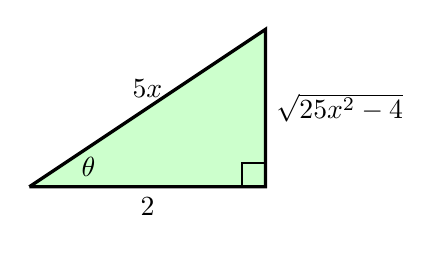
\begin{tikzpicture}
\draw [very thick, fill=green!20] (0,0) -- node[below,pos=.5] { $2$} (3,0) -- node [right,pos=.5] { $\sqrt{25x^2-4}$} (3,2) -- node [pos=.5,above] { $5x$} (0,0);
\draw [thick] (2.7,0) -- (2.7,.3) -- (3,.3);
\draw (.75,.25) node {$\theta$};			
\end{tikzpicture}
\end{center}
\end{minipage}
From the triangle, we get $ \ds \tan\theta = \frac{\sqrt{25x^2-4}}{2}  $.  
%$$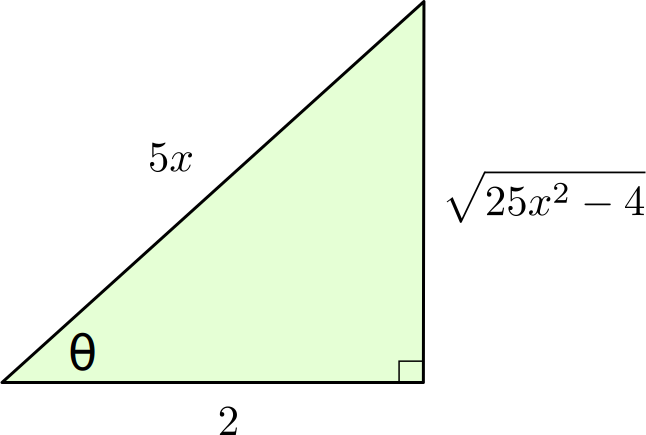
\includegraphics[height=1.5in]{images2/inv-trig-triangle-6}$$
As $\theta=\sec^{-1}(5x/2)$, we get
$$\ds\int\frac{\sqrt{25x^2-4}}{x}\,dx=2\left(\frac{\sqrt{25x^2-4}}{2}-\sec^{-1}\left(\frac{5x}{2}\right)\right)+C$$
\end{solution}

In the context of the previous example, some resources give alternate guidelines when choosing a trigonometric substitution.
\begin{center}\begin{tabular}{@{}ll@{}ll@{}}
	$\sqrt{a^2-b^2x^2}\quad\to\quad x=\ds\frac{a}{b}\sin\theta$\\
	\vspace{-0.1cm}\\
	$\sqrt{b^2x^2+a^2}~~\mbox{or}~~(b^2x^2+a^2)\quad\to\quad x=\ds\frac{a}{b}\tan\theta$\\
	\vspace{-0.1cm}\\
	$\sqrt{b^2x^2-a^2}\quad\to\quad x=\ds\frac{a}{b}\sec\theta$\\
\end{tabular}\end{center}

We next look at a tangent substitution.

%\begin{example}{Tangent Substitution}{Tangent Substitution}
%Evaluate $\ds\int\frac{1}{\sqrt{25+x^2}}\,dx$.
%\end{example}

%\begin{solution}
%Let $x=5\tan\theta$ so that $\fbox{$dx$}=\fbox{$5\sec^2\theta\,d\theta$}$.  
%$${\def\arraystretch{2.2}
%\begin{array}{>{\displaystyle}r>{\displaystyle}c>{\displaystyle}l>{\displaystyle}l}
%	\int\frac{1}{\sqrt{25+x^2}}\,\fbox{$dx$} & = & \int \frac{1}{\sqrt{25+25\tan^2\theta}}\,\fbox{$5\sec^2\theta\,d\theta$} &\mbox{Using our substitution}\\  
%	& = & \int\frac{1}{\sqrt{25(1+\tan^2\theta)}}\cdot5\sec^2\theta\,d\theta & \mbox{Factor out $25$}\\ 
%	& = & \int\frac{1}{5\sqrt{sec^2\theta}}\cdot5\sec^2\theta\,d\theta & \mbox{Using $\tan^2\theta+1=\sec^2\theta$}\\ 
%%	& = & \int\frac{1}{5\sec\theta}\cdot5\sec^2\theta\,d\theta & \mbox{Can ignore absolute value (why?)}\\ 
%	& = & \int\sec\theta\,d\theta & \mbox{Simplifying}\\ 
%	& = & \ln|\sec\theta+\tan\theta|+C & \mbox{By $\ds\int\sec \theta\,dx=\ln|\sec \theta+\tan \theta|+C$}\\
%\end{array}
%}$$
%Since $\tan\theta=x/5$, we draw a triangle:
%$$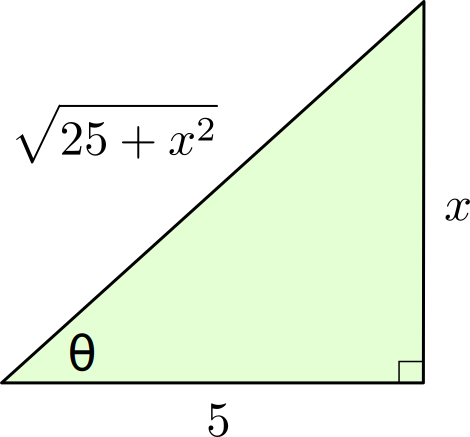
\includegraphics[height=1.5in]{images2/inv-trig-triangle-7}$$
%Then $$\ds\sec\theta=\frac{1}{\cos\theta}=\frac{\sqrt{25+x^2}}{5}.$$
%Therefore, the integral is
%$$\int\frac{1}{\sqrt{25+x^2}}\,dx=\ln\left|\frac{\sqrt{25+x^2}}{5}+\frac{x}{5}\right|+C$$
%\end{solution}


\begin{example}{Tangent Substitution}{Tangent Substitution}
Evaluate $\ds \int \frac{1}{\sqrt{5+x^2}}\ dx.$
\end{example}

\begin{solution}
Using part (b), we recognize $a=\sqrt{5}$ and  set $x= \sqrt{5}\tan \theta$. This makes $dx = \sqrt{5}\sec^2\theta\ d\theta$. We will use the fact that $\sqrt{5+x^2} = \sqrt{5+5\tan^2\theta} = \sqrt{5\sec^2\theta} = \sqrt{5}\sec\theta.$ Substituting, we have:
\begin{align*}
\int \frac{1}{\sqrt{5+x^2}}\ dx &= \int \frac{1}{\sqrt{5+5\tan^2\theta}}\sqrt{5}\sec^2\theta\ d\theta \\
			&= \int \frac{\sqrt{5}\sec^2\theta}{\sqrt{5}\sec\theta} \ d\theta\\
			&= \int \sec\theta\ d\theta\\
			&= \ln\big|\sec\theta+\tan\theta\big|+C.
\end{align*}
While the integration steps are over, we are not yet done. The original problem was stated in terms of $x$, whereas our answer is given in terms of $\theta$. We must convert back to $x$.

\begin{minipage}{.7\textwidth}
With $x=\sqrt{5}\tan\theta$, we have 
$$\tan \theta = \frac x{\sqrt{5}}\quad \text{and}\quad \sec\theta = \frac{\sqrt{x^2+5}}{\sqrt{5}}.$$
This gives
\end{minipage}
\begin{minipage}{.3\textwidth}
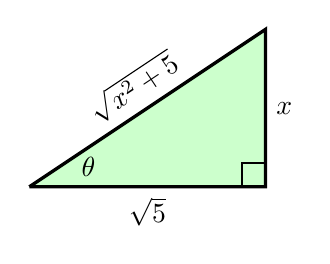
\begin{tikzpicture}
			\draw [very thick, fill=green!20] (0,0) -- node[below,pos=.5] { $\sqrt{5}$} (3,0) -- node [right,pos=.5] { $x$} (3,2) -- node [pos=.5,above,sloped] { $\sqrt{x^2+5}$} (0,0);
			\draw [thick] (2.7,0) -- (2.7,.3) -- (3,.3);
			\draw (.75,.25) node {$\theta$};	
	\end{tikzpicture}
\end{minipage}

\begin{align*}
\int \frac{1}{\sqrt{5+x^2}}\ dx &= \ln\big|\sec\theta+\tan\theta\big|+C \\
     &= \ln\left|\frac{\sqrt{x^2+5}}{\sqrt{5}}+ \frac x{\sqrt{5}}\right|+C.
\end{align*}
We can leave this answer as is, or we can use a logarithmic identity to simplify it. Note:
\begin{align*}
\ln\left|\frac{\sqrt{x^2+5}}{\sqrt{5}}+ \frac x{\sqrt{5}}\right|+C &= \ln\left|\frac{1}{\sqrt{5}}\big(\sqrt{x^2+5}+ x\big)\right|+C \\
   &= \ln\left|\frac{1}{\sqrt{5}}\right| + \ln\big|\sqrt{x^2+5}+ x\big|+C\\
	&=	\ln\big|\sqrt{x^2+5}+ x\big|+C,
\end{align*}
where the $\ln\big(1/\sqrt{5}\big)$ term is absorbed into the constant $C$. %(In Section \ref{sec:hyperbolic} we will learn another way of approaching this problem.)
\end{solution}

In the next example, we will use the technique of completing the square in order to rewrite the integrand.

\begin{example}{Completing the Square}{Completing the Square}
Evaluate $\ds\int\frac{x}{\sqrt{3-2x-x^2}}\,dx$.
\end{example}  

\begin{solution}
First, complete the square to write 
$$3-2x-x^2=4-(x+1)^2$$ 
Now, we may let $u=x+1$ so that $du=dx$ (note that $x=u-1$) to get:
$$\int\frac{x}{\sqrt{4-(x+1)^2}}\,dx=\int\frac{u-1}{\sqrt{4-u^2}}\,du$$ 
Let $u=2\sin\theta$ giving $du=2\cos\theta\,d\theta$: 
$$\int\frac{u-1}{\sqrt{4-u^2}}\,du = \int\frac{2\sin\theta-1}{2\cos\theta}\cdot 2\cos\theta\,d\theta=\int (2\sin\theta-1)\,d\theta$$
Integrating and using a triangle we get:
\begin{eqnarray*}
\int\frac{x}{\sqrt{3-2x-x^2}}	& = &-2\cos\theta-\theta+C  \\
	& = &-\sqrt{4-u^2}-\sin^{-1}\left(\frac{u}{2}\right)+C  \\
	& = &-\sqrt{3-2x-x^2}-\sin^{-1}\left(\frac{x+1}{2}\right)+C 
\end{eqnarray*}
Note that in this problem we could have skipped the $u$-substitution if instead we let $x+1=2\sin\theta$. (For the  triangle we would then use $\ds\sin\theta=\frac{x+1}{2}$.)
\end{solution}


%\bigskip
%\begin{example}{Another Inverse Sine Subsitution}{Another Inverse Sine Subsitution}\label{Another Inverse Sine Subsitution}
%Evaluate $\ds\int\sqrt{4-9x^2}\,dx$.
%\end{example}
%
%\begin{solution}
%We start by rewriting this so
%that it looks more like the previous example:
%$$
  %\int\sqrt{4-9x^2}\,dx=\int\sqrt{4(1-(3x/2)^2)}\,dx
  %=\int 2\sqrt{1-(3x/2)^2}\,dx.
%$$
%Now let $3x/2=\sin u$ so $(3/2)\,dx=\cos u \,du$ or
%$dx=(2/3)\cos u\,du$. Then
%\begin{eqnarray*}
%\int 2\sqrt{1-(3x/2)^2}\,dx&=&\int 2\sqrt{1-\sin^2u}\,(2/3)\cos u\,du\cr
%&=&{4\over3}\int \cos^2u\,du\cr
%&=&{4u\over 6}+{4\sin 2u\over12}+C\cr
%&=&{2\arcsin(3x/2)\over3}+{2\sin u \cos u\over3}+C\cr
%&=&{2\arcsin(3x/2)\over3}+{2\sin(\arcsin(3x/2))\cos(\arcsin(3x/2))\over3}+C\cr
%&=&{2\arcsin(3x/2)\over3}+{2(3x/2)\sqrt{1-(3x/2)^2}\over3}+C\cr
%&=&{2\arcsin(3x/2)\over3}+{x\sqrt{4-9x^2}\over2}+C,\cr
%\end{eqnarray*}
%using some of the work from example~\ref{Inverse Sine Subsitution}.
%\end{solution}
%
%
%
%\bigskip
%\begin{example}{Inverse Tangent Subsitution}{Inverse Tangent Subsitution}\label{Inverse Tangent Subsitution}
%Evaluate $\ds\int\sqrt{1+x^2}\,dx$.
%\end{example}
%
%\begin{solution}
%Let $x=\tan u$, 
%$\ds dx=\sec^2 u\,du$, so
%$$
  %\int\sqrt{1+x^2}\,dx=\int \sqrt{1+\tan^2 u}\sec^2u\,du=
  %\int\sqrt{\sec^2u}\sec^2u\,du.
%$$
%Since $u=\arctan(x)$, $-\pi/2\le u\le\pi/2$ and $\sec u\ge0$, so 
%$\ds \sqrt{\sec^2u}=\sec u$. Then
%$$\int\sqrt{\sec^2u}\sec^2u\,du=\int \sec^3 u \,du.$$
%Using the formula for the integral of $\sec^3 u$ and reverting to the original variable $x$:
%\begin{eqnarray*}
  %\int\sqrt{1+x^2}\,dx&=&{\sec u \tan u\over2}+{\ln|\sec u +\tan
    %u|\over2}+C\cr
  %&=&{\sec(\arctan x) \tan(\arctan x)\over2}
    %+{\ln|\sec(\arctan x) +\tan(\arctan x)|\over2}+C\cr
  %&=&{ x\sqrt{1+x^2}\over2}
    %+{\ln|\sqrt{1+x^2} +x|\over2}+C,\cr
%\end{eqnarray*}
%using $\tan(\arctan x)=x$ and 
%$\ds \sec(\arctan x)=\sqrt{1+\tan^2(\arctan x)}=\sqrt{1+x^2}$.
%\end{solution}


%%%%%%%%%%%%%%%%%%%%%%%%%%%%%%%%%%%%%%%%%%%%
\Opensolutionfile{solutions}[ex]
\section*{Exercises for \ref{sec:Trig Sub}}

\begin{enumialphparenastyle}

%%%%%%%%%%%
%\begin{ex}
 %$\ds\int\csc x\,dx$
%\begin{sol}
 %$-\ln|\csc x+\cot x|+C$
%\end{sol}
%\end{ex}
%%%%%%%%%%%
%
%%%%%%%%%%%
%\begin{ex}
 %$\ds\int\csc^3 x\,dx$
%\begin{sol}
 %$-\csc x\cot x/2-(1/2)\ln|\csc x+\cot x|+C$
%\end{sol}
%\end{ex}
%%%%%%%%%%%

%%%%%%%%%%
\begin{ex}
 $\ds\int\sqrt{x^2-1}\,dx$
\begin{sol}
 $\ds x\sqrt{x^2-1}/2-\ln|x+\sqrt{x^2-1}|/2+C$
\end{sol}
\end{ex}
%%%%%%%%%%

%%%%%%%%%%
\begin{ex}
 $\ds\int\sqrt{9+4x^2}\,dx$
\begin{sol}
 $\ds x\sqrt{9+4x^2}/2+\hbox{$\ds(9/4)\ln|2x+\sqrt{9+4x^2}|+C$}$
\end{sol}
\end{ex}
%%%%%%%%%%

%%%%%%%%%%
\begin{ex}
 $\ds\int x\sqrt{1-x^2}\,dx$
\begin{sol}
 $\ds -(1-x^2)^{3/2}/3+C$
\end{sol}
\end{ex}
%%%%%%%%%%

%%%%%%%%%%
\begin{ex}
 $\ds\int x^2\sqrt{1-x^2}\,dx$
\begin{sol}
 $\arcsin(x)/8-\sin(4\arcsin x)/32+C$
\end{sol}
\end{ex}
%%%%%%%%%%

%%%%%%%%%%
\begin{ex}
 $\ds\int{1\over\sqrt{1+x^2}}\,dx$
\begin{sol}
 $\ds \ln|x+\sqrt{1+x^2}|+C$
\end{sol}
\end{ex}
%%%%%%%%%%

%%%%%%%%%%
\begin{ex}
 $\ds\int\sqrt{x^2+2x}\,dx$
\begin{sol}
 $\ds (x+1)\sqrt{x^2+2x}/2-\hbox{$\ds\ln|x+1+\sqrt{x^2+2x}|/2+C$}$
\end{sol}
\end{ex}
%%%%%%%%%%

%%%%%%%%%%
\begin{ex}
 $\ds\int{1\over x^2(1+x^2)}\,dx$
\begin{sol}
 $-\arctan x - 1/x+C$
\end{sol}
\end{ex}
%%%%%%%%%%

%%%%%%%%%%
\begin{ex}
 $\ds\int{x^2\over\sqrt{4-x^2}}\,dx$
\begin{sol}
 $\ds 2\arcsin(x/2)-x\sqrt{4-x^2}/2+C$
\end{sol}
\end{ex}
%%%%%%%%%%

%%%%%%%%%%
\begin{ex}
 $\ds\int{\sqrt{x}\over\sqrt{1-x}}\,dx$
\begin{sol}
 $\ds \arcsin(\sqrt{x})-\sqrt{x}\sqrt{1-x}+C$
\end{sol}
\end{ex}
%%%%%%%%%%

%%%%%%%%%%
\begin{ex}
 $\ds\int{x^3\over\sqrt{4x^2-1}}\,dx$
\begin{sol}
 $\ds (2x^2+1)\sqrt{4x^2-1}/24+C$
\end{sol}
\end{ex}
%%%%%%%%%%

\end{enumialphparenastyle}